\section{Theorie}
\label{sec:Theorie}

Ziel des Versuches ist es die elastischen Konstanten eines Materiales zu bestimmen.
Außerdem soll das magnetische Moment eines permanent Magneten bestimmt werden. \\

In der Mechanik wird generell zwischen zwei Arten von Kräften unterschieden: 
Volumenkräfte, wie etwa die Gravitationskraft, bewirken eine Änderung des 
Bewegungszustandes, zum Beispiel eine Translation oder Rotation. 
Außerdem gibt es Oberflächenkräfte, die eine Gestalts- oder Volumenänderung 
bewirken. Die Kraft, die dabei auf einen Körper wirkt wird als Spannung bezeichnet. 
Eine senkrecht zum Körper angreifende Kraft wird als Normalspannung $\sigma$ benannt, 
eine die tangential zum Körper angreift als Tangentialspannung $\tau$. 

Für den Hookschen Bereich ist dabei die Kraft proportional zur Deformation, sodass 
elastische Konstanten zur Charakterisierung der Verformung eingeführt werden. 
Dieser Bereich zeichnet sich dadurch aus, dass dort Körper nach einer Deformation in 
ihren ursprünglichen Zustand zurückkehren. Es wird von einer "deelastischen 
Deformation" gesprochen. Für kleine Spannungen gilt also: 

\begin{equation*}
P = Q \frac{\symup{\Delta}V}{V}.
\end{equation*}

In einem Kristall mit niedriger Symmertrie werden jeweils 6 Komponenten für die 
Beschreibung der Deformation und Spannung benötigt. Daraus entsteht eine 6x6 Matrix 
mit insgesamt 36 Einträgen. Das Energieprinzip reduziert diese Anzahl allerdings 
aus 21 Komponenten, weitere lassen sich durch weitere Symmertrien eleminieren. 
In diesem Versuch werden nun isotrope Körper untersucht, wodurch sich die Anzahl 
auf zwei Konstanten verringert. Isotrope Körper zeichnen sich dadurch aus, dass die 
elastischen Konstanten richtungsunabhängig sind. 
Die benötigten Konstanten sind das Schubmodul $G$ für die Gestaltselastizität und 
das Kompressionsmodul $Q$ für die Volumenelastizität. Aus Gründen der Zweckmäßigkeit
werden außerdem der Elastizitätsmodul $E$ und die Poissonsche Querkontraktionszahl 
$\mu$ eingeführt. $E$ beschreibt dabei die relative Längenänderung beim Angreifen 
einer Normalspannung in Spannungsrichtung und $\mu$ die Längenänderung senkrecht 
zur Normalspannung. $\mu$ ist dabei definiert durch: 

\begin{equation*}
\mu = -\frac{\symup{\Delta}B}{B}\cdot \frac{L}{\symup{\Delta}L},
\end{equation*}

was durch Abbildung \ref{fig:Mu} verdeutlicht wird. 


\begin{figure}
  \centering
  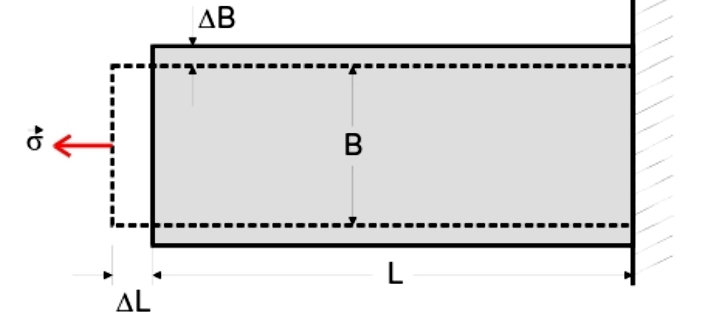
\includegraphics[scale=0.3]{content/Mu.png}
  \caption{Verdeutlichung der Querkontraktionszahl [1]}
  \label{fig:Mu}
\end{figure}

Zwischen den elastischen Konstanten $G$, $E$, $Q$ und $\mu$ gilt
der Zusammenhang: 

\begin{equation}
E = 2G(\mu +1) \leftrightarrow \mu = \frac{E}{2G} - 1
\end{equation}

\begin{equation}
E = 3(1-2\mu)Q \leftrightarrow Q = \frac{E}{3(1-2\mu)} \leftrightarrow Q = \frac{EG}{9G-\frac{3}{2}E}
\end{equation}

Bei Proben, die deutlich länger als breit sind, also $L>>B$ lassen sich der 
Elastizitätsmodul $E$ und Schubmodul $G$ besonders einfach bestimmen. Insbesondere
bei Metallen mit einem niedrigen Schmelzpunkt kommt es zu sogenannten 
elastischen Nachwirkungen. Damit wird bezeichnet, dass der ursprüngliche 
Zustand nicht unmittelbar nach der Verformung wieder eingenommen wird. 
Dies soll vermieden werden. 

\subsection{Bestimmung des Schubmoduls $G$}

Treten an einem Körper lediglich Tangentialspannungen auf, kommt es zu einer 
Scherung. Dabei wird der Körper in eine Richtung deformiert. Allerdings ist es 
sehr schwierig, den den sogenannten Scherungswinkel $\alpha$ zu bestimmen. 
Aus diesem Grund wird stattdessen die Torsion eines zylindrischen Stabes 
betrachtet. Dabei greifen an zwei gegenüberliegenden Punkten des Kreisdurchmessers
Kräfte in entgegengesetzten Richtungen an, wie in Abbildung \ref{fig:Torsion} dargestellt. 
Dies führt zu einer "Verzwirbelung" des
Probekörpers. Wird dieses Beispiel auf einen Draht projeziert, so wirkt nun
ein Drehmoment $M$ auf diesen. Dieses hängt auch von dem Hebelarm, also dem 
Abstand des Massepunktes von der Drehachse, ab. Die Variation über den 
Durchmesser hinweg, ergibt die Notwendigkeit den Körper in Holzylinder mit 
der infinitesimalen Dicke $dr$ und dem Radius $r$ zu zerlegen. 
Für das Drehmoment $M$ ergibt sich dadurch schließlich zu: 

\begin{equation}
M = \int_0^R 2\pi \frac{G}{L} \varphi r³ dr = \frac{\pi G R⁴ \varphi}{2 L}.
\end{equation}

Dabei ist R der Radius des Drahtes, L die Länge und $\varphi$ der Torsionswinkel. 

\begin{figure}
  \centering
  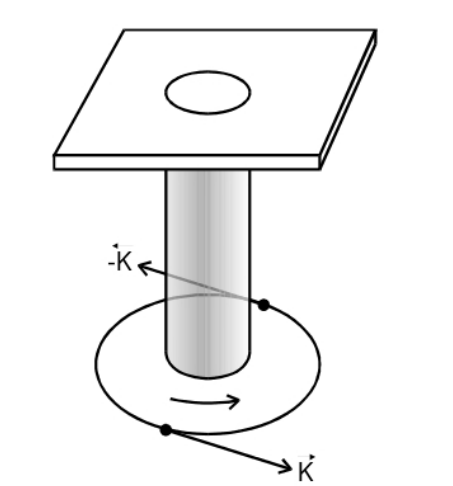
\includegraphics[scale=0.3]{content/Torsion.png}
  \caption{Verdeutlichung der Torsion [1]}
  \label{fig:Torsion}
\end{figure}

Somit lautet die Richtgröße $D$:

\begin{equation}
D = \frac{\pi G R⁴}{2 L}.
\end{equation}

Angesprochene Nachwirkungen werden vermieden durch eine Messmethode, 
bei der die Spannung eine periodische Funktion der Zeit ist. Dafür 
wird eine Kugel an den Draht gehängt und ausgelenkt. Durch die entgegengesetzt
wirkenden Drehmomente kommt es zu einer Drehschwingung. 
Es ergibt sich eine Differentialgleichung zweiter Ordnung, die durch einen 
Cosinusansatz gelöst wird. Dadurch ergibt sich für die Periodendauer $T$
folgender Zusammenhang: 

\begin{equation}
T = 2\pi \sqrt{\frac{\theta}{D}}
\label{eqn:Periode}
\end{equation}

Dabei bezeichnet $\theta$ das Trägheitsmoment der Kugel. Dieses ist im 
Allgemeinem gegeben durch: 

\begin{equation*}
\theta_\text{K} = \frac{2}{5} m_\text{K}R_\text{K}²
\end{equation*}

$m_\text{K}$ ist dabei gegeben als Masse der Kugel und $R_\text{K}$ als Radius
der Kugel. Wird $\theta_\text{K}$ und $D$ in \eqref{eqn:Periode} eingesetzt ergibt sich: 

\begin{equation*}
T = 2\pi \sqrt{\frac{4Lm_\text{K}R_\text{K}²}{5\pi GR⁴}}
\end{equation*}

Umformen zu G führt zu: 

\begin{equation}
G = \frac{16\pi m_\text{K} R_\text{K}² L}{5T²R⁴}
\end{equation}

\subsection{Bestimmung des magnetischen Momentes des Permanentmagneten}

Für die Bestimmung des magnetischen Momentes eines Permanentmagneten ist 
folgende Beziehung gegeben: 

\begin{equation*}
\vec{m} = p \vec{a}
\end{equation*}

mit $p$ als Polstärke und $a$ als Abstand der Pole, der von Nord- zum Südpol 
zeigt. In einem homogenen B-Feld wirken auf den Magneten zwei entgegengesetzte
Kräfte, was in Abbildung \ref{fig:Magnet} veranschaulicht wird. Diese Kräfte sind entgegengesetzt
durch das unterschiedliche Vorzeichen von $p$. Es wirkt also ein magnetisches 
Drehmoment, dass betraglich durch

\begin{equation}
M_\text{mag} = m B \sin{\gamma}
\end{equation}

gegeben ist. 

\begin{figure}
  \centering
  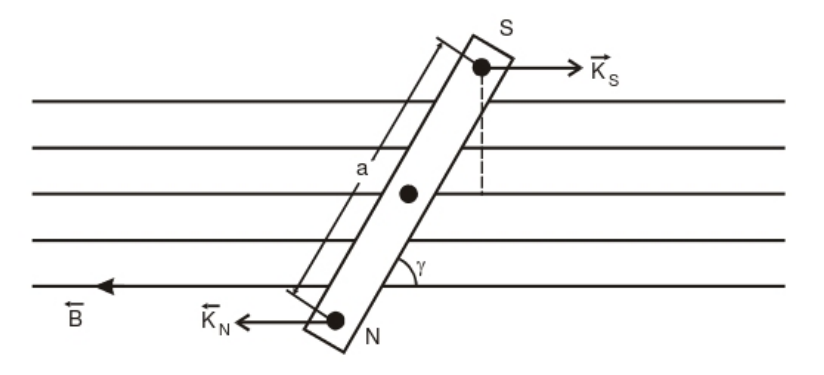
\includegraphics[scale=0.3]{content/Magnet.png}
  \caption{Permanentmagnet in einem äußeren Magnetfeld $\vec{B}$ [1]}
  \label{fig:Magnet}
\end{figure}

Die nicht-lineare Differentialgleichung wird durch eine Kleinwinkelnäherung linearisiert
und lässt sich ebenfalls durch einen Cosinusansatz lösen. Daraus ergibt sich die Periodendauer
bei aktivierten Magnetfeld und daraus widerrum das magnetische Moment $m$.

\begin{equation}
T = 2\pi \sqrt{\frac{\theta}{mB+D}} \leftrightarrow m = \frac{4\pi²\theta}{BT²}-\frac{D}{B}
\end{equation}